\chapter{研究背景}

\section{问题提出}

跨媒介职业转型已经成为东亚娱乐产业中的常见现象。传统纸媒时代，职业晋升更多依赖杂志封面、广告代言与电视剧曝光；进入视频平台时代后，艺人需要在更高频的互动环境中持续解释自我、修复争议并管理公众期待\cite{Jenkins2006,Goffman1959}。因此，“转型”不再只是职业名称的改变，而是生产机制与传播机制同时变化的结果。

`projects/NSFC_Young` 当前示例关注东亚艺人职业路径与品牌韧性的研究价值，本公开 thesis 示例沿用这一主题，但将其扩展为一篇结构完整的硕士论文，以验证毕业论文模板在封面、摘要、目录、章节、图表、缩略词表和致谢等环节上的稳定性。

\section{理论基础}

\subsection{职业生命周期视角}

Super 的职业发展理论强调，个体在探索、建立、维持和再适应之间不断移动\cite{Super1957}。在娱乐产业中，这一过程往往被平台变化进一步放大：当媒介形式更新时，原有声誉资本并不会自动转化为新平台优势。

\subsection{形象管理视角}

Goffman 的“自我呈现”理论指出，公众人物需要在不同场景中组织可接受的角色形象\cite{Goffman1959}。当社交媒体和短视频平台进入职业系统后，这种呈现从阶段性展示转变为持续性协商，危机也更容易转化为长期标签。

\section{案例价值}

佐佐木希的公开职业轨迹兼具三个特点。第一，职业阶段足够长，能够覆盖传统媒体与新媒体两种生产逻辑。第二，角色类型跨越模特、演员、综艺嘉宾与视频创作者，可用于展示“同一主体的多次转型”。第三，危机事件与重启过程均有公开资料，便于构建可重复的案例编码框架。

\begin{figure}[H]
  \centering
  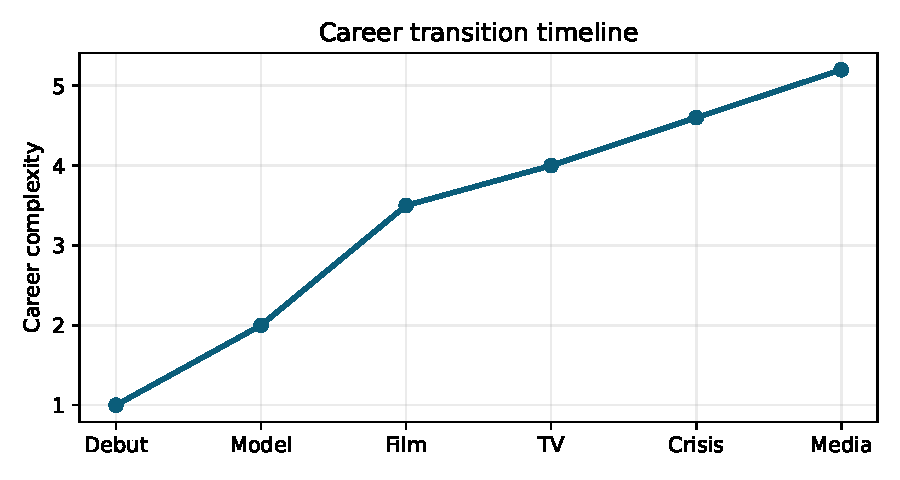
\includegraphics[width=0.82\textwidth]{assets/demo/transition-timeline.pdf}
  \caption{示例案例的职业转型时间线}
  \label{fig:smu-timeline}
\end{figure}

\section{研究问题}

围绕上述背景，本示例提出三个问题：

\begin{enumerate}
  \item 跨媒介职业转型可以划分为哪些稳定阶段？
  \item 传统媒体积累的可见度如何转化为新媒体中的可控叙事能力？
  \item 危机后的品牌韧性是否可以用公开指标做出结构化描述？
\end{enumerate}

\section{研究设计概览}

\figref{fig:smu-timeline} 所示时间线用于展示“阶段划分”能力；后续章节再分别用表格、长表格与结果图展示编码框架、指标设定与韧性评分的呈现方式。通过这种安排，模板的主要样式均可在公开内容中得到覆盖。
